\chapter{Segmentation}

\section{Where?}
\begin{itemize}
\item Used in the identification of anatomical structures, lesions, or regions of interest.
\item Example: 3D surface reconstruction (ultrasound).
\end{itemize}
  
\section{Types of segmentation}

\begin{itemize}
\item \textbf{Semantic}: Find objects inside an image and classify them according to predetermined categories.
\item \textbf{Instance}: Distinguish amount the object of the same category.
\item \textbf{Panoptic}: A particular case of instance segmentation where all the pixels of the image are classified.
\end{itemize}

\begin{figure}[H]
  \vspace{-0ex}
  \centering
  \href{https://www.labellerr.com/blog/semantic-vs-instance-vs-panoptic-which-image-segmentation-technique-to-choose/}{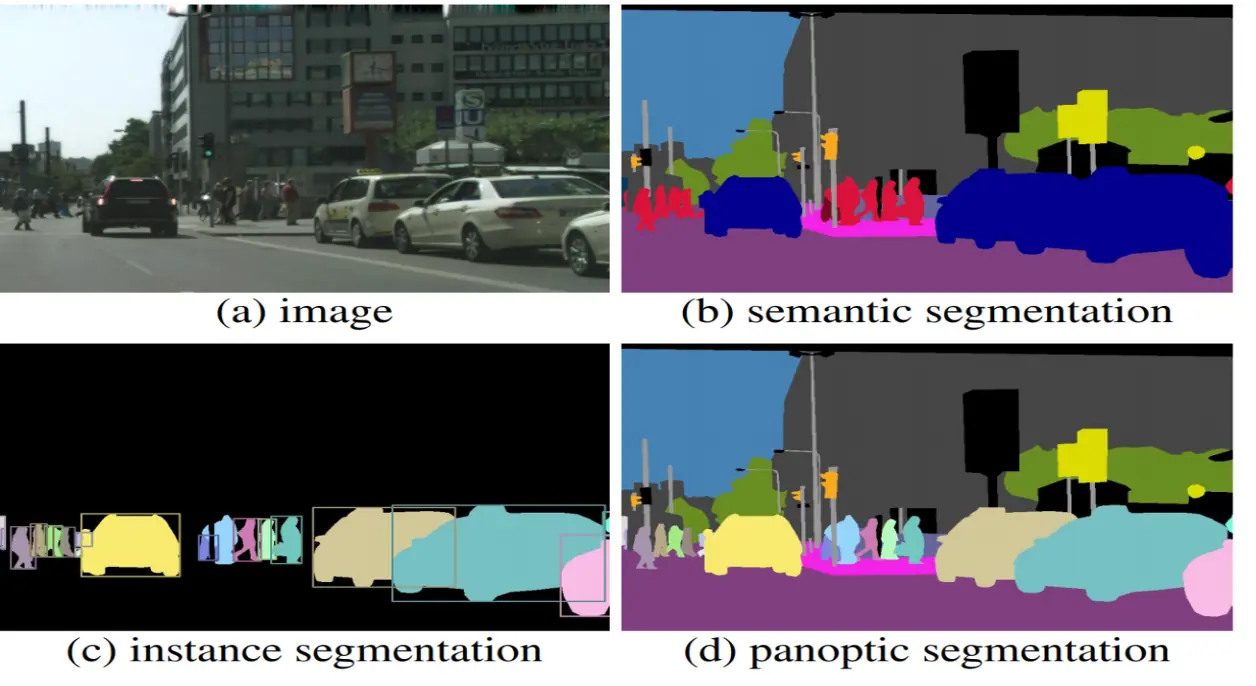
\includegraphics[width=0.9\textwidth]{semantic_vs_instance_vs_panoptic}}
  \caption{Types of segmentation.}
  \label{fig:types_segmentation}
\end{figure}

\section{Thresholding \cite{gonzalez2009digital}}
\begin{itemize}
\item Decide the classification by comparing the $I(x,y)$ pixel values with a threshold $t$, generating the binarized image
  \begin{equation}
    O(x,y) = \begin{cases*}
      1 & {\text if}\quad $I(x,y)>t$ \\
      0 & {\text otherwise}
    \end{cases*} 
  \end{equation}
  where $O(x,y)$ are the output pixel values.
\end{itemize}

\begin{figure}[H]
  \vspace{1ex}
  \centering
\href{https://github.com/vicente-gonzalez-ruiz/medical_imaging/blob/main/notebooks/thresholding.ipynb}{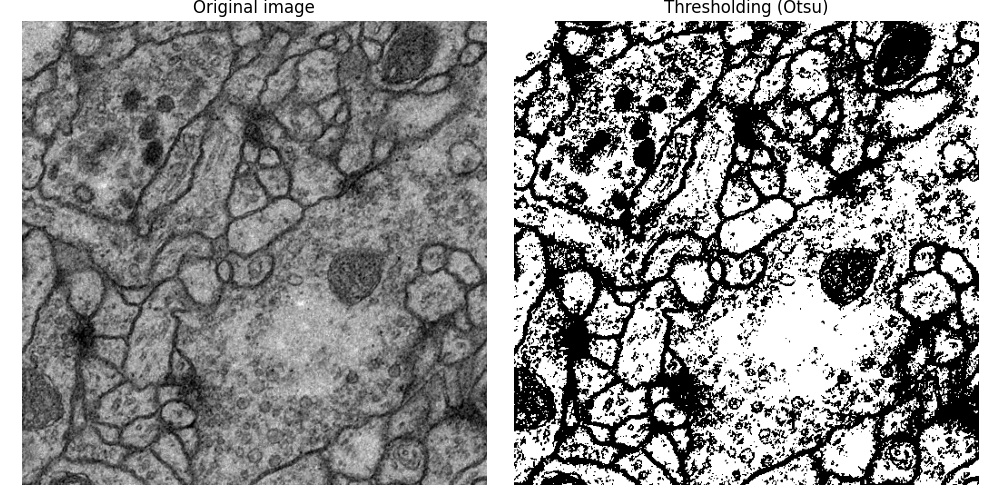
\includegraphics[width=0.9\textwidth]{thresholding}}
  \caption[An example of segmentation by thresholding.]{An example of
    segmentation by thresholding. Otsu is used for selection the
    threshold value.}
  \label{fig:thresholding}
\end{figure}

\section{U-Net segmentation \cite{ronneberger2015u}}

\begin{itemize}
\item A machine learning technique based on a deep \gls{CNN} (see Section~\ref{sec:UNet}).
\item Supervised learning (the training set must be labeled).
\end{itemize}

%\href{https://github.com/byrkbrk/unet-implementation?tab=readme-ov-file}{unet-implementation}

%\begin{center}
%  \href{https://github.com/vicente-gonzalez-ruiz/medical_imaging/blob/main/notebooks/unet_cell_data.ipynb}{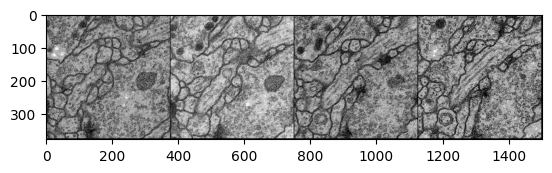
\includegraphics[width=12cm]{unet_cell_data}}
%  \href{https://github.com/vicente-gonzalez-ruiz/medical_imaging/blob/main/notebooks/unet_cell_data.ipynb}{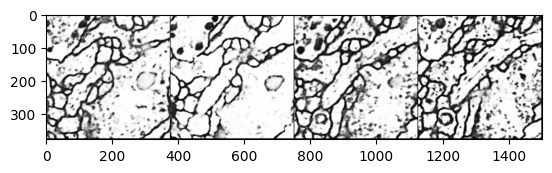
\includegraphics[width=12cm]{unet_cell_data_result}}
%\end{center}

\begin{figure}[H]
  \vspace{1ex}
  \centering
\href{https://github.com/vicente-gonzalez-ruiz/medical_imaging/blob/main/notebooks/unet_cell_data.ipynb}{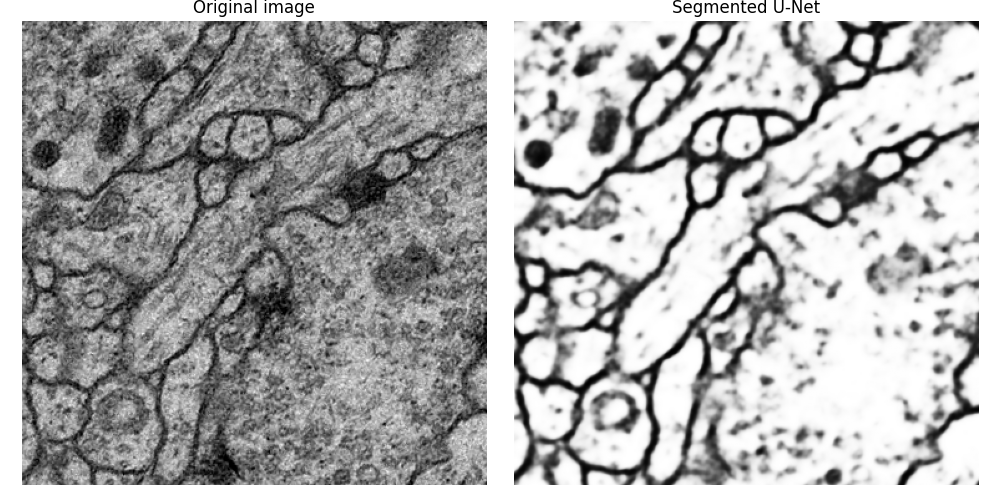
\includegraphics[width=0.9\textwidth]{U-Net_segmentation}}
  \caption[An example of segmentation using a U-Net.]{An example of
    segmentation using a U-Net. Only a crop is shown.}
  \label{fig:U-Net_segmentatin}
\end{figure}

